\section{Camera}

\begin{definition}
The \emph{camera} functions as an optical sensor, generating data through electric transducers. 
It incorporates an optical system that directs incoming light at each of its millions of photosensitive elements. 
Modern cameras typically have the capability to record 30 to 60 frames per second.
\end{definition}
For the sake of simplicity, we assume that the optical system of a camera consists of a single lens with the following characteristics:
\begin{itemize}
    \item \textit{Spherical}: the lens is created by the intersection of two spherical surfaces.
    \item \textit{Thin}: the distance between the centers of the two spheres is nearly equal to the sum of their radius.
    \item \textit{Small angles}: the light rays make only slight inclinations with respect to the optical axis.
\end{itemize}
These simplifications facilitate the calculation of the path of a ray as it passes through the lens.
Specifically, the refraction of light when it crosses the boundary between two media is governed by Snell's law:
\[\dfrac{\sin{\theta_2}}{\sin{\theta_1}}=\dfrac{n_1}{n_2}\]
Here: 
\begin{itemize}
    \item $\theta_1$ and $\theta_2$ represent the angles between the normal at the surface and the direction of the light ray before and after crossing the boundary, respectively.
    \item $n_1$ and $n_2$ are the refractive indices of the two materials.
\end{itemize}
\begin{figure}[H]
    \centering
    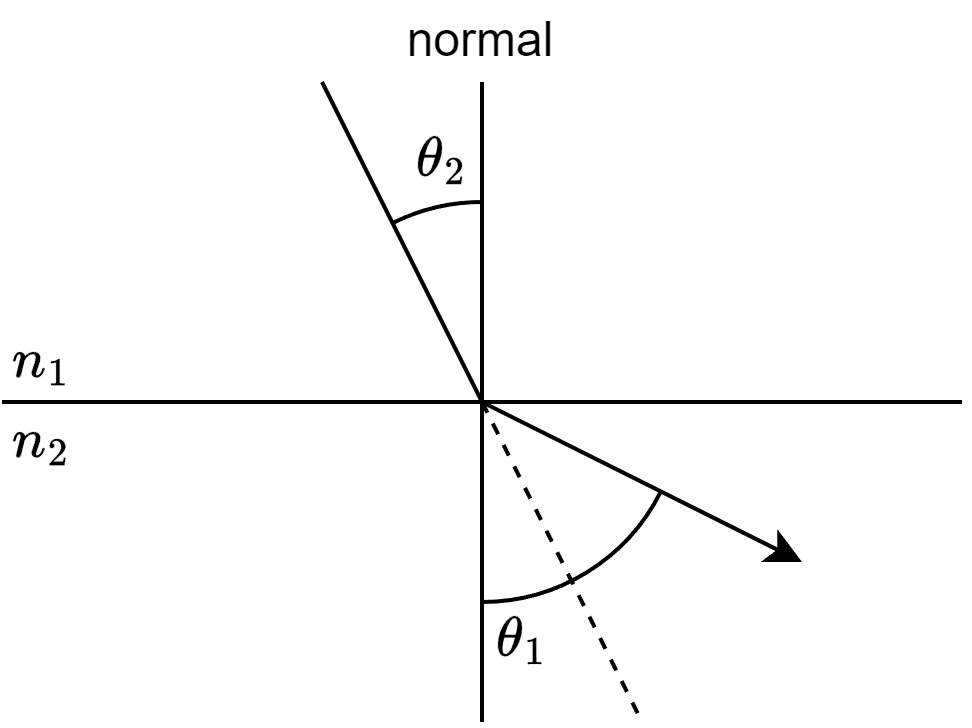
\includegraphics[width=0.4\linewidth]{images/refraction.png}
    \caption{Snell's law}
\end{figure}
\begin{definition}
    The \emph{optical axis} is the straight line that connects the center of the two spheres that compose the lens.
\end{definition}
The angles of a ray passing through the centers of the spheres can be determined as follows:
\[\alpha_1=\dfrac{y_1}{\rho_1} \:\:\:\:\:\: \alpha_2=-\dfrac{y_2}{\rho_2}\]
\begin{figure}[H]
    \centering
    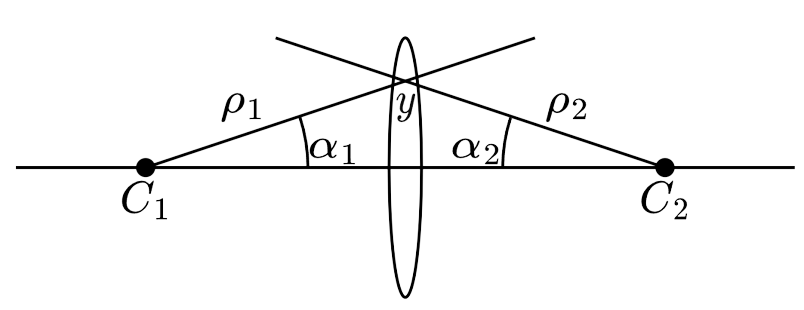
\includegraphics[width=0.4\linewidth]{images/y.png}
\end{figure}
In this context, with a simplified lens, it's valid to assume:
\[y_1=y_2=y\]